% TRM (Tiny Recursive Model) architecture — MLP-mixer Sudoku variant, as run in exp_a01/a02 (#73).
% Style matches the "Permutations Are All You Need" paper figures (box/proj/op/stream node styles,
% Stealth arrows, dashed loop-returns). Standalone-compilable: pdflatex trm_architecture.tex
\documentclass[border=8pt]{standalone}
\usepackage{amsmath,amssymb}
\usepackage{xcolor}
\usepackage{tikz}
\usetikzlibrary{positioning, arrows.meta, fit, calc, backgrounds, shapes.geometric}
\begin{document}
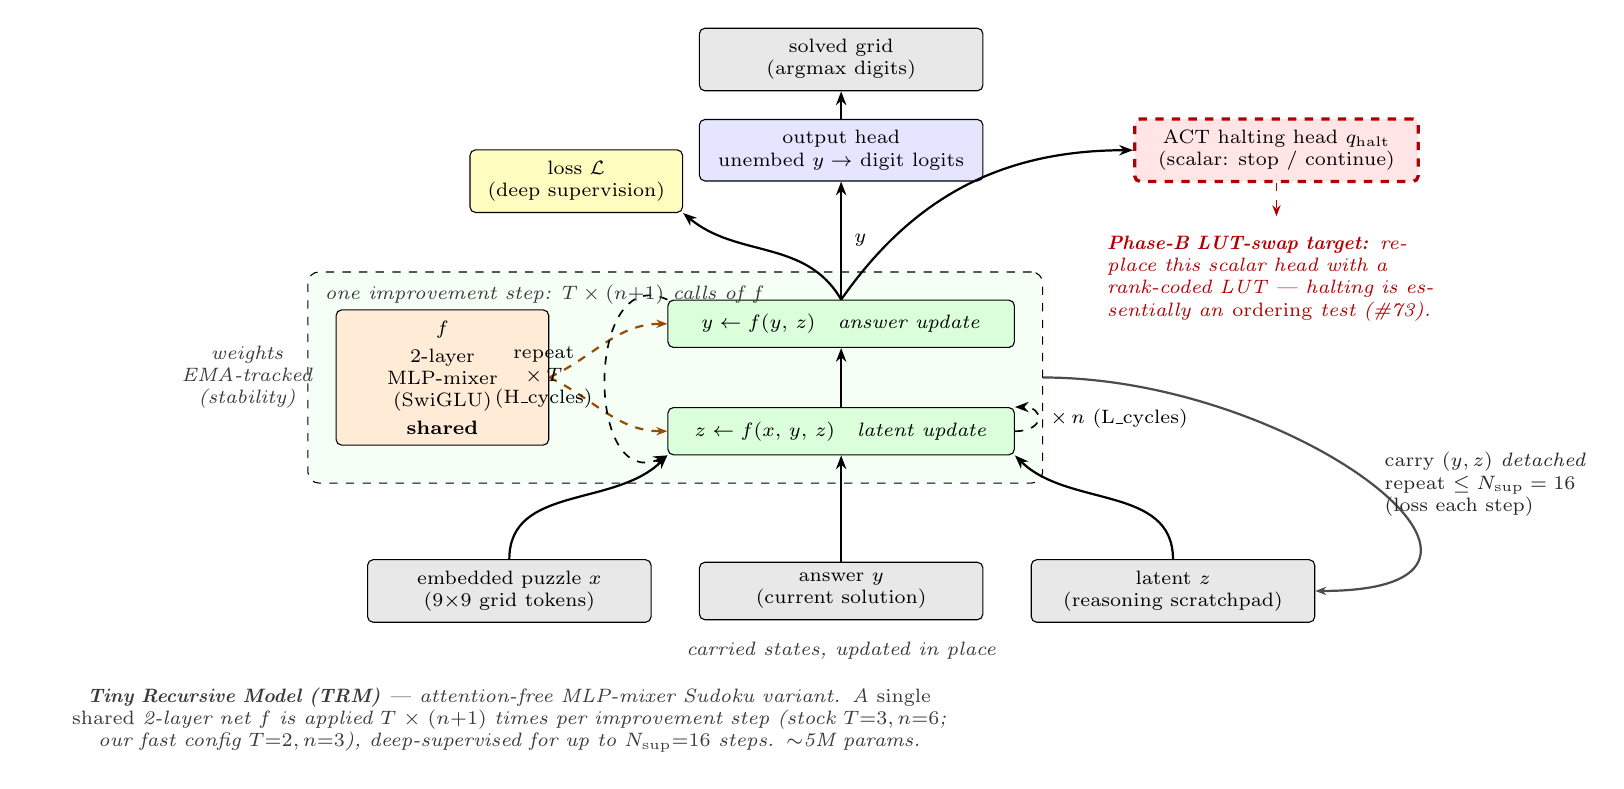
\begin{tikzpicture}[
    every node/.style={font=\scriptsize},
    box/.style={rectangle, draw, rounded corners=2pt, align=center, inner sep=4pt, fill=#1, minimum height=0.6cm, minimum width=3.6cm},
    box/.default=blue!8,
    proj/.style={box=blue!10},
    stream/.style={box=gray!18},
    op/.style={box=green!14, minimum width=4.4cm},
    net/.style={rectangle, draw, rounded corners=2pt, align=center, inner sep=4pt, fill=orange!16, minimum height=1.7cm, minimum width=2.7cm},
    lut/.style={rectangle, draw=red!70!black, dashed, very thick, rounded corners=2pt, align=center, inner sep=4pt, fill=red!10, minimum height=0.6cm, minimum width=3.6cm},
    loss/.style={box=yellow!25, minimum width=2.7cm},
    arr/.style={-{Stealth[length=5pt]}, thick},
    looparr/.style={-{Stealth[length=5pt]}, semithick, dashed},
    share/.style={-{Stealth[length=4pt]}, thick, orange!60!black, dashed},
    sidearr/.style={-{Stealth[length=4pt]}, thick, gray!60!black},
    callout/.style={font=\scriptsize\itshape, align=left, text=red!70!black},
    lbl/.style={font=\scriptsize\itshape, align=center, text=gray!45!black},
]

% ---------- inputs (bottom row) ----------
\node[stream] (x) {embedded puzzle $x$\\\scriptsize(9$\times$9 grid tokens)};
\node[stream, right=0.6cm of x] (y0) {answer $y$\\\scriptsize(current solution)};
\node[stream, right=0.6cm of y0] (z0) {latent $z$\\\scriptsize(reasoning scratchpad)};
\node[lbl, below=0.15cm of y0] {carried states, updated in place};

% ---------- recursion core ----------
\node[op, above=1.35cm of y0] (zupd) {$z \leftarrow f(x,\,y,\,z)$\quad\emph{latent update}};
\node[op, above=0.75cm of zupd] (yupd) {$y \leftarrow f(y,\,z)$\quad\emph{answer update}};

% shared tiny network, to the left, feeding both updates (weight sharing)
\coordinate (mid) at ($(zupd.west)!0.5!(yupd.west)$);
\node[net, left=1.5cm of mid] (f) {$f$\\[2pt]2-layer\\MLP-mixer\\(SwiGLU)\\[2pt]\textbf{shared}};
\draw[share] (f.east) to[out=-25,in=180] (zupd.west);
\draw[share] (f.east) to[out=25,in=180] (yupd.west);
\node[lbl, left=0.05cm of f, text width=1.9cm, anchor=east] (ema) {weights\\EMA-tracked\\(stability)};

% self-loop: inner latent loop repeated n times
\draw[looparr] (zupd.east) to[out=0,in=0,looseness=3.2] node[right=1pt,midway,text=black]{$\times\,n$\ \scriptsize(L\_cycles)} (zupd.east |- zupd.north);

% wrap the whole improvement pass T times (H_cycles)
\draw[looparr] (yupd.north west) to[out=155,in=-155,looseness=1.5]
    node[left=1pt,midway,text=black,align=center]{repeat\\$\times\,T$\\\scriptsize(H\_cycles)} (zupd.south west);

% feed inputs into the recursion
\draw[arr] (x.north) to[out=90,in=-135] (zupd.south west);
\draw[arr] (y0.north) -- (zupd.south);
\draw[arr] (z0.north) to[out=90,in=-45] (zupd.south east);
\draw[arr] (zupd) -- (yupd);

% box around the improvement step
\begin{scope}[on background layer]
\node[draw, dashed, rounded corners=4pt, fill=green!4, inner sep=10pt,
      fit=(zupd)(yupd)(f)] (step) {};
\end{scope}
\node[lbl, anchor=north west] at ($(step.north west)+(0.1,-0.05)$)
     {one improvement step: $T\times(n{+}1)$ calls of $f$};

% ---------- deep supervision (outer loop) ----------
\node[loss, above left=1.1cm and -0.2cm of yupd] (loss) {loss $\mathcal{L}$\\\scriptsize(deep supervision)};
\draw[arr] (yupd.north) to[out=120,in=-40] (loss.south east);
% outer loop return: carry (y,z) detached back to the states, up to N_sup steps
\draw[sidearr] (step.east) to[out=0,in=0,looseness=1.9]
    node[right=1pt,midway,align=left,text=gray!30!black]{carry $(y,z)$ \emph{detached}\\repeat $\le N_{\mathrm{sup}}=16$\\(loss each step)} (z0.east);

% ---------- heads (top) ----------
\node[proj, above=1.5cm of yupd] (ohead) {output head\\\scriptsize unembed $y \to$ digit logits};
\node[stream, above=0.35cm of ohead] (logits) {solved grid\\\scriptsize(argmax digits)};
\draw[arr] (yupd.north) -- (ohead) node[midway,right=1pt]{$y$};
\draw[arr] (ohead) -- (logits);

% halting head + Phase-B LUT callout
\node[lut, right=1.9cm of ohead] (qhalt) {ACT halting head $q_{\mathrm{halt}}$\\\scriptsize(scalar: stop / continue)};
\draw[arr] (yupd.north) to[out=55,in=180] (qhalt.west);
\node[callout, below=0.55cm of qhalt, text width=4.3cm, anchor=north]
     {\textbf{Phase-B LUT-swap target:} replace this scalar head with a rank-coded LUT --- halting is essentially an \emph{ordering} test (\#73).};
\draw[-{Stealth[length=4pt]}, dashed, red!70!black] (qhalt.south) -- ++(0,-0.42);

% ---------- title / caption strip ----------
\node[lbl, below=0.7cm of x, text width=12cm, anchor=north]
     {\textbf{Tiny Recursive Model (TRM)} --- attention-free MLP-mixer Sudoku variant.
      A \emph{single shared} 2-layer net $f$ is applied $T\times(n{+}1)$ times per improvement step
      (stock $T{=}3,n{=}6$; our fast config $T{=}2,n{=}3$), deep-supervised for up to
      $N_{\mathrm{sup}}{=}16$ steps. $\sim$5M params.};

\end{tikzpicture}
\end{document}
